\section{Test}
Vi har kørt vores implementation med de 3 udleverede programmer.\\

Med alle sideudskiftningsalgoritmer er programmerne kørt med 100 siders virtuel hukommelse og fra 10 til 100 rammer fysisk hukommelse, med trin af 10 rammer. Dette har resulteret i følgende statistikker:

\begin{figure}[H]
	\centering
	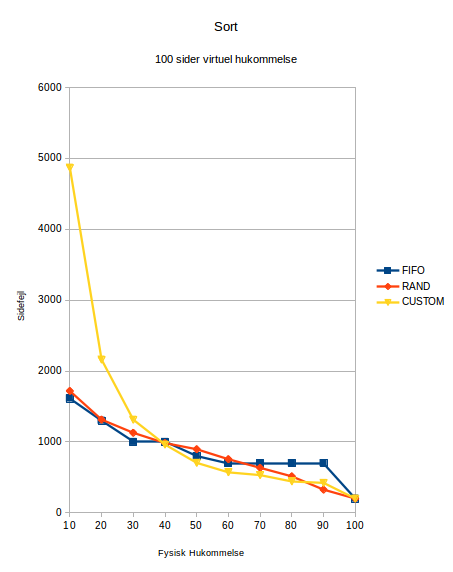
\includegraphics[width=0.8\textwidth]{figures/SortStatistic.png}
	\caption{Kørsler af Sort-programmet. Figuren viser de 3 sideudskiftningsalgoritmers antal af sidefejl holdt op mod antallet af rammer i den fysiske hukommelse.}
	\label{fig:sortstatistic}
\end{figure}

Som det ses i Figur \ref{fig:sortstatistic} er den brugerdefinerede sideudskiftningsalgoritme ikke effektiv i situationer hvor der er meget begrænset fysisk hukommelse, og hukommelsen bliver tilgået meget spredt.\\

Dog når den brugerdefinerede algoritme hurtigt ned på samme antal fejl, når antallet af rammer stiger en smule. Algoritmen bliver dog overhalet på antal fejl af den tilfældige algoritme, når mængden af fysisk hukommelse nærmer sig mængden af virtuel hukommelse.\\

\begin{figure}[H]
	\centering
	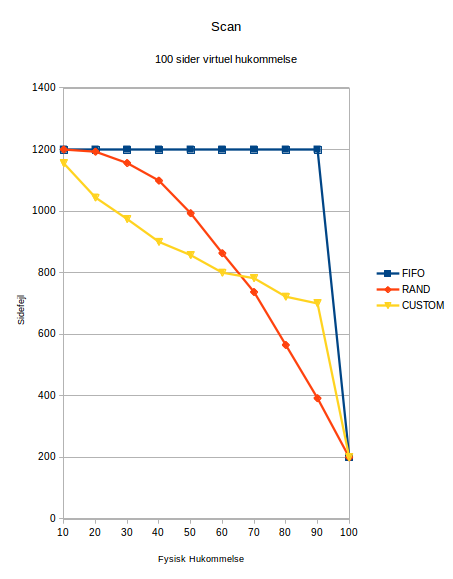
\includegraphics[width=0.8\textwidth]{figures/ScanStatistic.png}
	\caption{Kørsler af Scan-programmet. Figuren viser de 3 sideudskiftningsalgoritmers antal af sidefejl holdt op mod antallet af rammer i den fysiske hukommelse.}
	\label{fig:scanstatistic}
\end{figure}

I Figur \ref{fig:scanstatistic} ses det at den brugerdefinerede algoritme klarer sig bedst i situationer hvor den fysiske hukommelse er op til 60 \% af den virtuelle hukommelse. Herefter bliver den dog overhalet af den tilfældige algoritme, hvis der ses på antallet af sidefejl.\\

\begin{figure}[H]
	\centering
	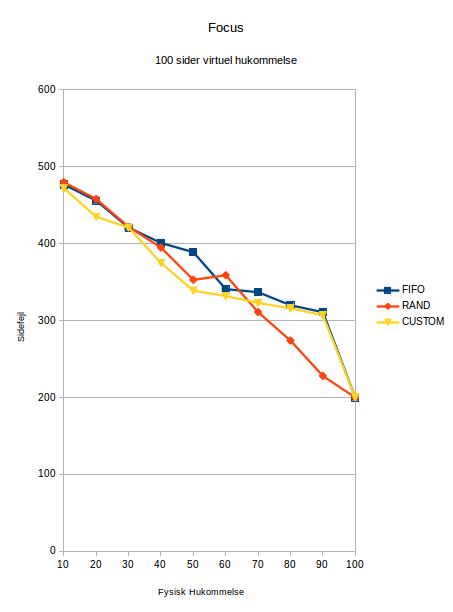
\includegraphics[width=0.8\textwidth]{figures/FocusStatistic.png}
	\caption{Kørsler af Focus-programmet. Figuren viser de 3 sideudskiftningsalgoritmers antal af sidefejl holdt op mod antallet af rammer i den fysiske hukommelse.}
	\label{fig:focusstatistic}
\end{figure}

I Figur \ref{fig:focusstatistic} er den brugerdefinerede algoritme omtrent lige så god som de andre (marginalt bedre), indtil den fysiske hukommelse er ca. 70 \% af den virtuelle hukommelse. Herefter fører den tilfældige algoritme igen.\\

Det er drmed ikke lykkedes at skabe en algoritme der altid kan opnå færre sidefejl end de 2 andre i \textit{alle} situationer. Dog ses det, at når den fysiske hukommelse er halvt så stor som den virtuelle, fører den brugerdefinerede algoritme marginalt.\\

\begin{figure}[H]
	\centering
	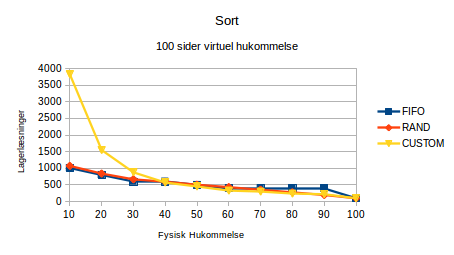
\includegraphics[width=0.85\textwidth]{figures/SortReads.png}	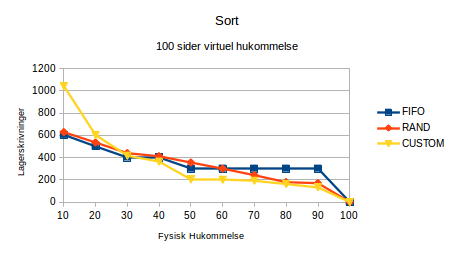
\includegraphics[width=0.85\textwidth]{figures/SortWrites.png}	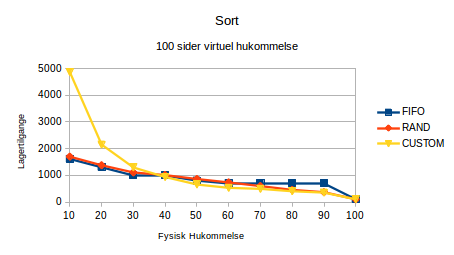
\includegraphics[width=0.85\textwidth]{figures/SortAccess.png}
	\caption{Kørsler af Sort-programmet. De 3 diagrammer viser henholdsvis lagerlæsninger, lagerskrivninger, og lagertilgange. Det sidste diagram er altså en sum af de 2 forrige.}
	\label{fig:sortdisk}
\end{figure}

\begin{figure}[H]
	\centering
	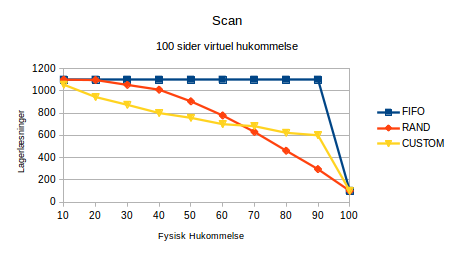
\includegraphics[width=0.85\textwidth]{figures/ScanReads.png}	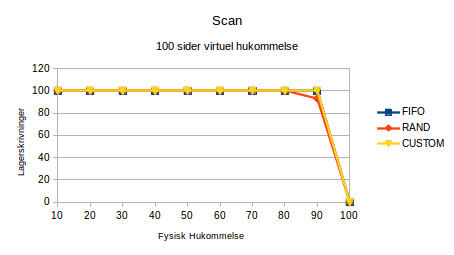
\includegraphics[width=0.85\textwidth]{figures/ScanWrites.png}	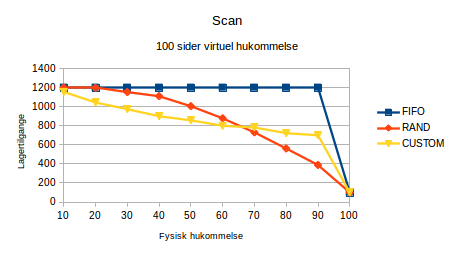
\includegraphics[width=0.85\textwidth]{figures/ScanAccess.png}
	\caption{Kørsler af Scan-programmet. De 3 diagrammer viser henholdsvis lagerlæsninger, lagerskrivninger, og lagertilgange. Det sidste diagram er altså en sum af de 2 forrige.}
	\label{fig:scandisk}
\end{figure}

\begin{figure}[H]
	\centering
	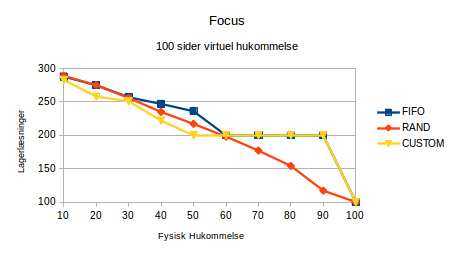
\includegraphics[width=0.85\textwidth]{figures/FocusReads.png}	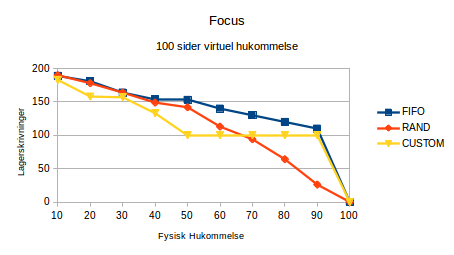
\includegraphics[width=0.85\textwidth]{figures/FocusWrites.png}	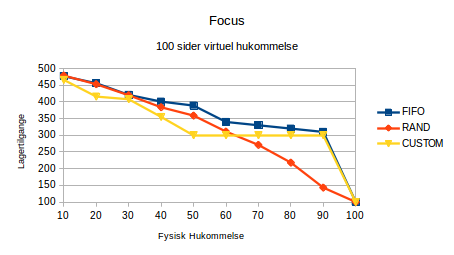
\includegraphics[width=0.85\textwidth]{figures/FocusAccess.png}
	\caption{Kørsler af Focus-programmet. De 3 diagrammer viser henholdsvis lagerlæsninger, lagerskrivninger, og lagertilgange. Det sidste diagram er altså en sum af de 2 forrige.}
	\label{fig:focusdisk}
\end{figure}

I diagrammerne på figur \ref{fig:sortdisk}, \ref{fig:scandisk} og \ref{fig:focusdisk} ses det, at tilgangen til lageret stemmer nogenlunde overens med antallet af sidefejl, som beskrevet tidligere. Særligt i de to første figurer ses det, at antallet af læsninger overstiger antallet af skrivninger for alle sideudskiftningsalgoritmerne. Derfor bruger den brugerdefinerede algoritme, ligesom pagefaults, altså færre drevtilgange end kø implementationen og den tilfældige implementation ved omkring 50\% størrelse af det fysiske lager i forhold til den virtuelle hukommelse. I mange tilfælde er den bedre end køen ved mere end 50\% fysisk hukommelse.